\chapter{Hardware and Softwarestack}\label{ch:hardware-and-softwarestack}


\section{Overview}\label{sec:overview}

The mobile application will be developed for Android and tested using a Google Pixel 7.
It will be coded in Kotlin using Android Studio.

The Google ARCore API will be used to access depth information about a scene.
The API is available by default -- no additional libraries are required.

Algorithms will be implemented in C\texttt{++} in the \texttt{procedural-augmented-reality} project provided by Prof. Dr. Phillipp Jenke.
The project will be embedded into the application and will be called through a binding layer from Kotlin.


\section{Google ARCore SDK}

ARCore is an Augmented Reality (AR) software development kit (SDK) designed by Google for multiple platforms including Android.
It supports multiple tools like motion tracking, anchor tracking, surface tracking, depth perception and light estimation.
\parencite{arcore}
For the purposes of the topic of this thesis, depth understanding is the most important part,
as it provides depth information which can be used to run algorithms for primitive detection on.

\subsection{Depth API}
Googles documentation~\parencite{arcore-doc-depth} summarizes the features of the Depth API the following way:

\textit{
    The Depth API uses a depth-from-motion algorithm to create depth images, which give a 3D view of the world.
    Each pixel in a depth image is associated with a measurement of how far the scene is from the camera.
    This algorithm takes multiple device images from different angles and compares them to estimate the distance to every pixel as a user moves their phone.
    It selectively uses machine learning to increase depth processing, even with minimal motion from a user.
    It also takes advantage of any additional hardware a user’s device might have.
    If the device has a dedicated depth sensor, such as ToF, the algorithm automatically merges data from all available sources.
}

The device used for development (Google Pixel 7) is not equipped with a depth sensor, thus the Depth API will solely rely on cameras depth-from-motion to generate depth information.
The inherent pitfall of camera based depth-from-motion is that tracking objects with little to no texture like walls will not yield good result.
This might pose challenges, depending on the specific use case to be examined in the thesis.
If, for example, objects like boxes or spheres with little to no texture are to be recognized,
the depth API might not return sufficiently accurate depth information to correctly recognize them.

\subsubsection{API Details}
The Depth API provides the two APIs, as described by \citetitle{arcore-doc-raw-depth}~\parencite{arcore-doc-raw-depth}:
\begin{enumerate}
    \item The Raw Depth API provides "raw depth images that contain a very accurate depth estimate for some, but not all, pixels in the camera image."
    It also provides a "confidence image that gives the confidence for every raw depth images pixel".
    \item The Full Depth API provides a "single 'smoothed' depth image that contains a depth estimate for every pixel."
\end{enumerate}

Example images of the two APIs can be seen in figure~\ref{fig:depth-api-images}

The Raw Depth API seems to be the better choice for the use case of analyzing 3D data, as it provides more accurate data.
The choice between the APIs needs to be investigated further for the final implementation.

\subsubsection{Calculating 3D Point Cloud based on Depth Images}
As the Depth API returns depth images and not point clouds, every pixel needs to be projected into 3D space using the camera intrinsics.
The~\citetitle[p. 5]{arcore-codelab-rawdepth} provides an example implementation called \textit{convertRawDepthImagesTo3dPointBuffer} that solves this problem.



\begin{figure}[ht!]
    \centering
    % First row
    \begin{subfigure}[b]{0.4\textwidth}
        \centering
        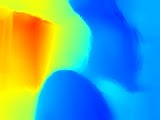
\includegraphics[width=0.8\linewidth]{images/depth_full-depth-image}
        \caption{Full Depth API Depth Image}
    \end{subfigure}%
    \begin{subfigure}[b]{0.4\textwidth}
        \centering
        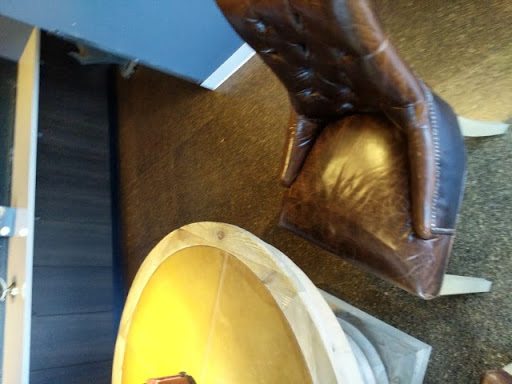
\includegraphics[width=0.8\linewidth]{images/depth_camera-image}
        \caption{Camera image}
    \end{subfigure}%

    % Optional: Adjust or remove vertical spacing between the rows
    \vspace{0.5em}

    % Second row
    \begin{subfigure}[b]{0.4\textwidth}
        \centering
        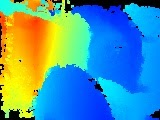
\includegraphics[width=0.8\linewidth]{images/depth_raw-depth-image}
        \caption{Raw Depth API Depth Image}
    \end{subfigure}%
    \begin{subfigure}[b]{0.4\textwidth}
        \centering
        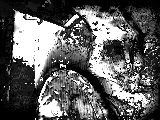
\includegraphics[width=0.8\linewidth]{images/depth_raw-depth-confidence-image}
        \caption{Raw Depth API Confidence Image}
    \end{subfigure}%

    \caption{Full Depth vs. Raw Depth}
    \label{fig:depth-api-images}
\end{figure}

\subsection{Confirming Compatibility with Device}

The quickstart section of the documentation of the \citetitle{arcore-depth-quickstart}~\parencite{arcore-depth-quickstart} provides a sample application named \texttt{hello\_ar\_kotlin}.
The \texttt{hello\_ar\_kotlin} application has been confirmed to run on the hardware mentioned in section~\ref{sec:overview}.
Screenshots of the running sample application can be seen in figure~\ref{fig:hello_world_screenshot}.


\begin{figure}[ht!]
    \centering
    \begin{subfigure}[t]{.45\textwidth}
        \centering
        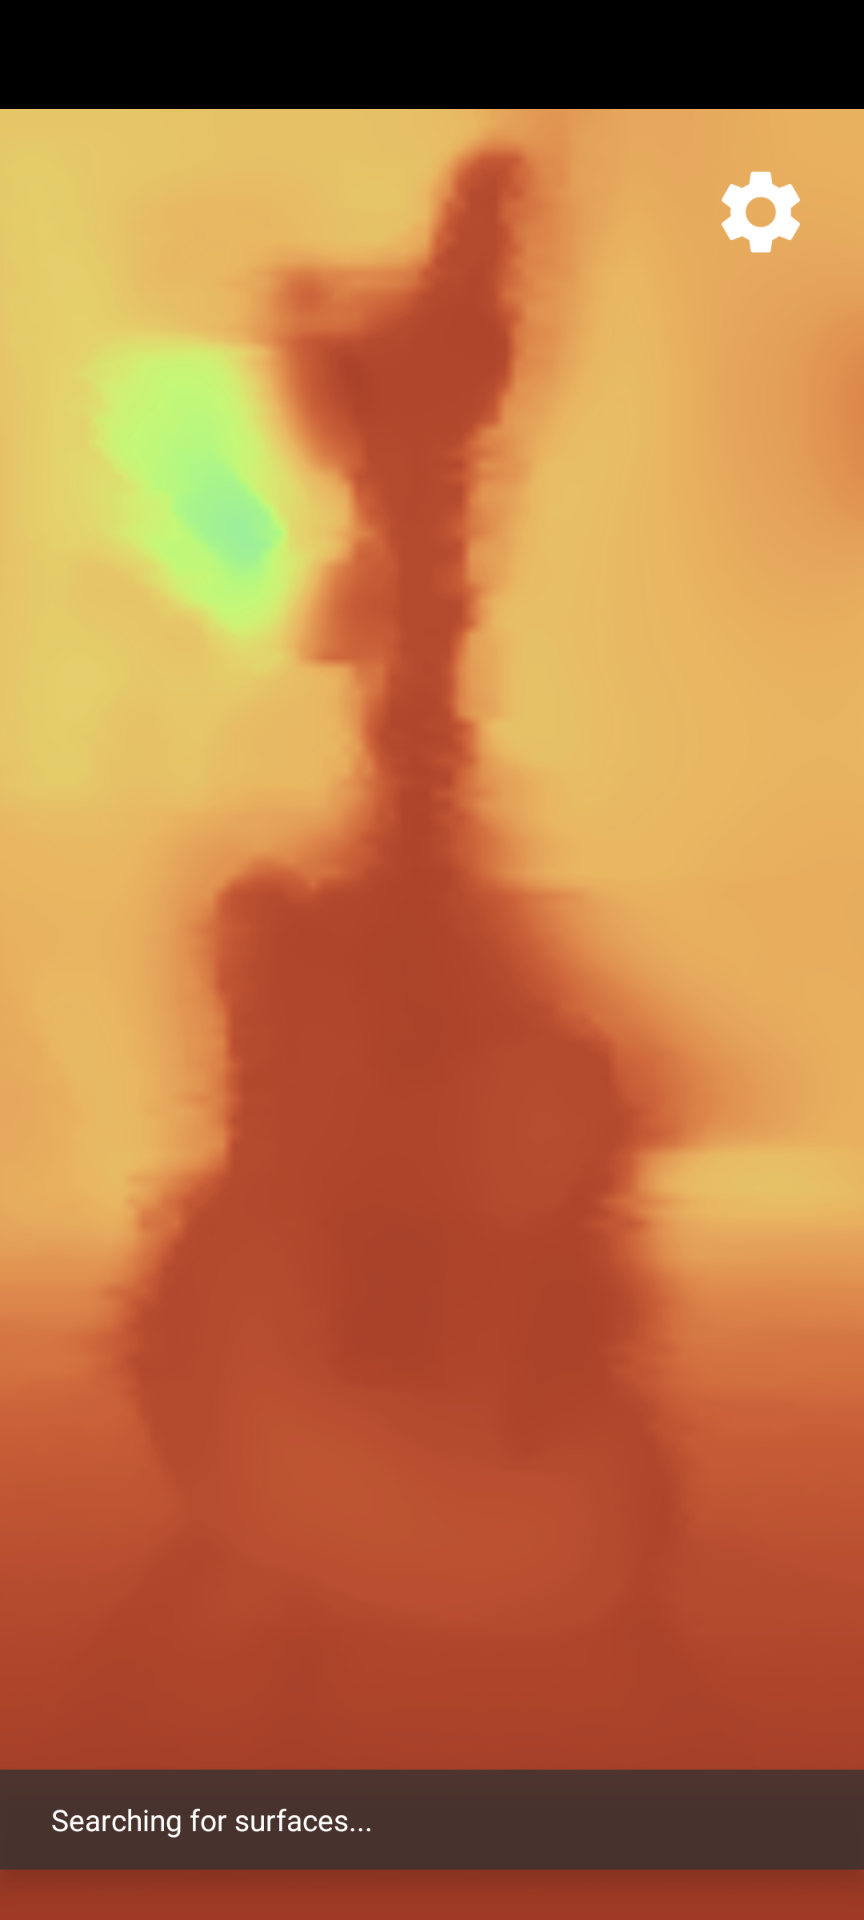
\includegraphics[width=.8\textwidth]{images/depth_api_hello_world_depth}
        \caption{Depth image, colors represent depth}
    \end{subfigure}\hfill
    \begin{subfigure}[t]{.45\textwidth}
        \centering
        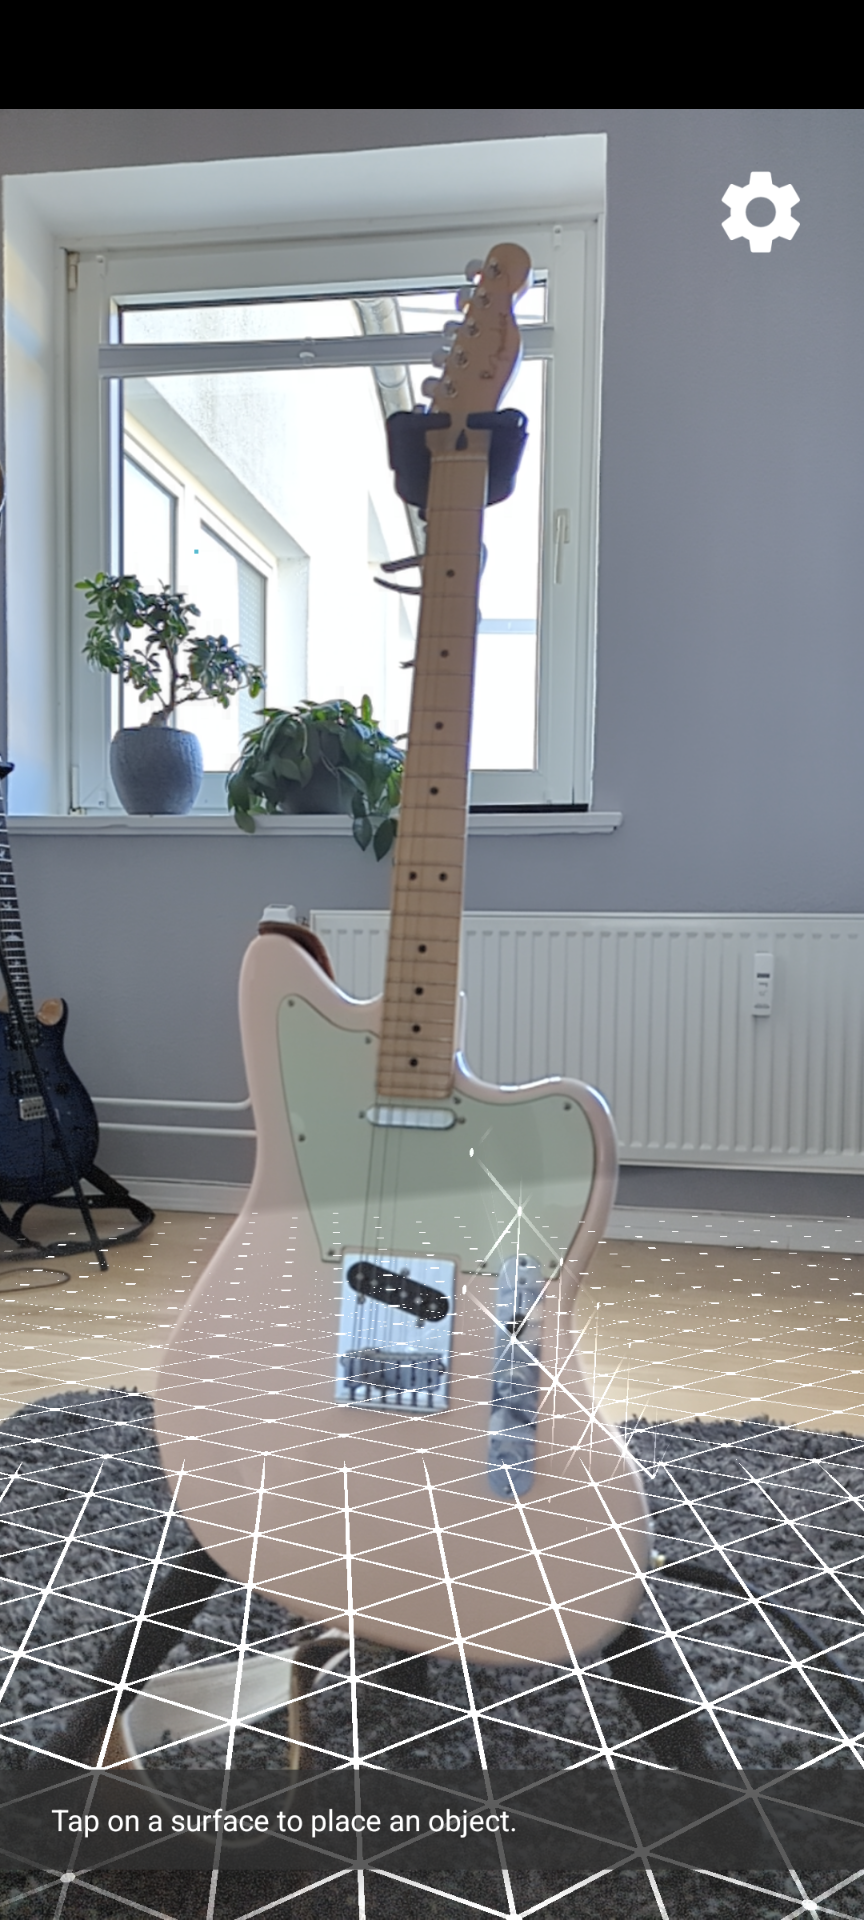
\includegraphics[width=.8\textwidth]{images/depth_api_hello_world_img}
        \caption{Full color reference. Floor is recognized as surface.}
    \end{subfigure}
    \caption{Screenshots of the \texttt{hello\_ar\_kotlin} sample application running on a Google Pixel 7}
    \label{fig:hello_world_screenshot}
\end{figure}
